\documentclass[11pt,]{article}
\usepackage[left=1in,top=1in,right=1in,bottom=1in]{geometry}
\newcommand*{\authorfont}{\fontfamily{phv}\selectfont}
  \usepackage[]{mathpazo}
  
  
  \usepackage[T1]{fontenc}
\usepackage[utf8]{inputenc}



\usepackage{abstract}
\renewcommand{\abstractname}{}    % clear the title
\renewcommand{\absnamepos}{empty} % originally center

\renewenvironment{abstract}
{{%
  \setlength{\leftmargin}{0mm}
  \setlength{\rightmargin}{\leftmargin}%
}%
  \relax}
{\endlist}

\makeatletter
\def\@maketitle{%
  \newpage
  %  \null
  %  \vskip 2em%
    %  \begin{center}%
    \let \footnote \thanks
  {\fontsize{18}{20}\selectfont\raggedright  \setlength{\parindent}{0pt} \@title \par}%
}
%\fi
\makeatother


  
  
  \setcounter{secnumdepth}{0}

      \usepackage{color}
  \usepackage{fancyvrb}
  \newcommand{\VerbBar}{|}
  \newcommand{\VERB}{\Verb[commandchars=\\\{\}]}
  \DefineVerbatimEnvironment{Highlighting}{Verbatim}{commandchars=\\\{\}}
  % Add ',fontsize=\small' for more characters per line
  \usepackage{framed}
  \definecolor{shadecolor}{RGB}{248,248,248}
  \newenvironment{Shaded}{\begin{snugshade}}{\end{snugshade}}
  \newcommand{\AlertTok}[1]{\textcolor[rgb]{0.94,0.16,0.16}{#1}}
  \newcommand{\AnnotationTok}[1]{\textcolor[rgb]{0.56,0.35,0.01}{\textbf{\textit{#1}}}}
  \newcommand{\AttributeTok}[1]{\textcolor[rgb]{0.77,0.63,0.00}{#1}}
  \newcommand{\BaseNTok}[1]{\textcolor[rgb]{0.00,0.00,0.81}{#1}}
  \newcommand{\BuiltInTok}[1]{#1}
  \newcommand{\CharTok}[1]{\textcolor[rgb]{0.31,0.60,0.02}{#1}}
  \newcommand{\CommentTok}[1]{\textcolor[rgb]{0.56,0.35,0.01}{\textit{#1}}}
  \newcommand{\CommentVarTok}[1]{\textcolor[rgb]{0.56,0.35,0.01}{\textbf{\textit{#1}}}}
  \newcommand{\ConstantTok}[1]{\textcolor[rgb]{0.00,0.00,0.00}{#1}}
  \newcommand{\ControlFlowTok}[1]{\textcolor[rgb]{0.13,0.29,0.53}{\textbf{#1}}}
  \newcommand{\DataTypeTok}[1]{\textcolor[rgb]{0.13,0.29,0.53}{#1}}
  \newcommand{\DecValTok}[1]{\textcolor[rgb]{0.00,0.00,0.81}{#1}}
  \newcommand{\DocumentationTok}[1]{\textcolor[rgb]{0.56,0.35,0.01}{\textbf{\textit{#1}}}}
  \newcommand{\ErrorTok}[1]{\textcolor[rgb]{0.64,0.00,0.00}{\textbf{#1}}}
  \newcommand{\ExtensionTok}[1]{#1}
  \newcommand{\FloatTok}[1]{\textcolor[rgb]{0.00,0.00,0.81}{#1}}
  \newcommand{\FunctionTok}[1]{\textcolor[rgb]{0.00,0.00,0.00}{#1}}
  \newcommand{\ImportTok}[1]{#1}
  \newcommand{\InformationTok}[1]{\textcolor[rgb]{0.56,0.35,0.01}{\textbf{\textit{#1}}}}
  \newcommand{\KeywordTok}[1]{\textcolor[rgb]{0.13,0.29,0.53}{\textbf{#1}}}
  \newcommand{\NormalTok}[1]{#1}
  \newcommand{\OperatorTok}[1]{\textcolor[rgb]{0.81,0.36,0.00}{\textbf{#1}}}
  \newcommand{\OtherTok}[1]{\textcolor[rgb]{0.56,0.35,0.01}{#1}}
  \newcommand{\PreprocessorTok}[1]{\textcolor[rgb]{0.56,0.35,0.01}{\textit{#1}}}
  \newcommand{\RegionMarkerTok}[1]{#1}
  \newcommand{\SpecialCharTok}[1]{\textcolor[rgb]{0.00,0.00,0.00}{#1}}
  \newcommand{\SpecialStringTok}[1]{\textcolor[rgb]{0.31,0.60,0.02}{#1}}
  \newcommand{\StringTok}[1]{\textcolor[rgb]{0.31,0.60,0.02}{#1}}
  \newcommand{\VariableTok}[1]{\textcolor[rgb]{0.00,0.00,0.00}{#1}}
  \newcommand{\VerbatimStringTok}[1]{\textcolor[rgb]{0.31,0.60,0.02}{#1}}
  \newcommand{\WarningTok}[1]{\textcolor[rgb]{0.56,0.35,0.01}{\textbf{\textit{#1}}}}
        
    \usepackage{graphicx,grffile}
\makeatletter
\def\maxwidth{\ifdim\Gin@nat@width>\linewidth\linewidth\else\Gin@nat@width\fi}
\def\maxheight{\ifdim\Gin@nat@height>\textheight\textheight\else\Gin@nat@height\fi}
\makeatother
% Scale images if necessary, so that they will not overflow the page
% margins by default, and it is still possible to overwrite the defaults
% using explicit options in \includegraphics[width, height, ...]{}
\setkeys{Gin}{width=\maxwidth,height=\maxheight,keepaspectratio}
  
    \title{Homework 5  }
  
  
  
  \author{\Large Joyce Yu Cahoon\vspace{0.05in} \newline\normalsize\emph{}  }
  
  
  \date{}

\usepackage{titlesec}

\titleformat*{\section}{\normalsize\bfseries}
\titleformat*{\subsection}{\normalsize\itshape}
\titleformat*{\subsubsection}{\normalsize\itshape}
\titleformat*{\paragraph}{\normalsize\itshape}
\titleformat*{\subparagraph}{\normalsize\itshape}


  
      
  
  \newtheorem{hypothesis}{Hypothesis}
\usepackage{setspace}

\makeatletter
\@ifpackageloaded{hyperref}{}{%
  \ifxetex
  \PassOptionsToPackage{hyphens}{url}\usepackage[setpagesize=false, % page size defined by xetex
                                                 unicode=false, % unicode breaks when used with xetex
                                                 xetex]{hyperref}
  \else
    \PassOptionsToPackage{hyphens}{url}\usepackage[unicode=true]{hyperref}
  \fi
}

\@ifpackageloaded{color}{
  \PassOptionsToPackage{usenames,dvipsnames}{color}
}{%
  \usepackage[usenames,dvipsnames]{color}
}
\makeatother
\hypersetup{breaklinks=true,
bookmarks=true,
pdfauthor={Joyce Yu Cahoon ()},
pdfkeywords = {},  
pdftitle={Homework 5},
colorlinks=true,
citecolor=blue,
urlcolor=blue,
linkcolor=magenta,
pdfborder={0 0 0}}
\urlstyle{same}  % don't use monospace font for urls

% set default figure placement to htbp
\makeatletter
\def\fps@figure{htbp}
\makeatother

\setlength{\abovedisplayskip}{.2pt}
\setlength{\belowdisplayskip}{.2pt}
\usepackage{placeins}
\usepackage{setspace}
\usepackage{chngcntr}
\usepackage{multicol}
\usepackage{lscape}
\counterwithin{figure}{section}
\counterwithin{table}{section}
\usepackage{mathrsfs}
\usepackage{mathtools}
\usepackage{multirow}
\newtheorem{theorem}{Theorem}
\usepackage[linesnumbered,algoruled,boxed,lined,commentsnumbered]{algorithm2e}
\usepackage{bm}
\usepackage{framed}
\usepackage{xcolor}
\let\oldquote=\quote
\let\endoldquote=\endquote
\colorlet{shadecolor}{orange!15}
\renewenvironment{quote}{\begin{shaded*}}{\end{shaded*}}
\newcommand{\minus}{\scalebox{0.75}[1.0]{$-$}}
\newcommand{\V}[1]{{\bm{{#1}}}}


% add tightlist ----------
\providecommand{\tightlist}{%
\setlength{\itemsep}{0pt}\setlength{\parskip}{0pt}}

\begin{document}

% \pagenumbering{arabic}% resets `page` counter to 1 
%
% \maketitle

{% \usefont{T1}{pnc}{m}{n}
\setlength{\parindent}{0pt}
\thispagestyle{plain}
{\fontsize{18}{20}\selectfont\raggedright 
\maketitle  % title \par  

}

{
  \vskip 13.5pt\relax \normalsize\fontsize{11}{12} 
  \textbf{\authorfont Joyce Yu Cahoon} \hskip 15pt \emph{\small }   
  
}

}






\vskip 6.5pt


\noindent  \hypertarget{section}{%
\section{7.7}\label{section}}

Show that the solution to 7.18 is given by 7.17. As a further
generalization, what is the solution to the following problem:
minimizing with respect the symmetric matrix \({\bm{{S}}}\):

\[
||\hat{{\bm{{\Sigma}}}}_{\lambda} - {\bm{{S}}}||^2_{F} \quad \text{such that} \quad \lambda_{\min}({\bm{{S}}}) \geq \delta
\]

We can show the solution to 7.18 is given by 7.17 since: \[
\begin{aligned}
||\hat{{\bm{{\Sigma}}}}_{\lambda} - {\bm{{S}}}||^2_{F} &= tr[(\hat{{\bm{{\Sigma}}}}_{\lambda} - {\bm{{S}}})(\hat{{\bm{{\Sigma}}}}_{\lambda} - {\bm{{S}}})^T] \\
&= tr(\hat{{\bm{{\Sigma}}}}\hat{{\bm{{\Sigma}}}}^T) - tr(\hat{{\bm{{\Sigma}}}} {\bm{{S}}}^T) - tr({\bm{{S}}} \hat{{\bm{{\Sigma}}}}^T) + tr({\bm{{S}}}{\bm{{S}}}^T) \\
&= tr(\hat{{\bm{{\Sigma}}}} \hat{{\bm{{\Sigma}}}}^T) - 2tr(\hat{{\bm{{\Sigma}}}} {\bm{{S}}}^T) +  tr({\bm{{S}}}{\bm{{S}}}^T) 
\end{aligned}
\] Since we eventually want to constrain \({\bm{{S}}}\) to positive
definite matrices, let's represent \({\bm{{S}}}\) as
\({\bm{{V}}}{\bm{{V}}}^T\), leading to: \[
\begin{aligned}
tr(\hat{{\bm{{\Sigma}}}} \hat{{\bm{{\Sigma}}}}^T) - 2tr(\hat{{\bm{{\Sigma}}}} {\bm{{S}}}{\bm{{S}}}^T) +  tr({\bm{{V}}}{\bm{{V}}}^T{\bm{{V}}}{\bm{{V}}}^T) 
\end{aligned}
\] Taking the derivative of this relative to \({\bm{{V}}}\) results in
\(-4{\bm{{V}}}^T\hat{{\bm{{\Sigma}}}} + 4{\bm{{V}}}^T{\bm{{V}}}{\bm{{V}}}^T = 0\).
We can simplify and solve this by letting
\({\bm{{V}}} = \Gamma^T ({\Lambda}^+)^{1/2}\). Since our covariance
matrix is symmetric and can be broken down into
\(\Gamma^T \Lambda \Gamma\), then: \[
\begin{gathered}
-4[(\Lambda^+)^{1/2} \Gamma \Gamma^T (\Lambda^+ + \Lambda^-)\Gamma] + 4(\Lambda^+)^{1/2}\Gamma \Gamma^T (\Lambda^+)^{1/2} (\Lambda^+)^{1/2} \Gamma \\ 
-4[(\Lambda^+)^{1/2} (\Lambda^+ + \Lambda^-) \Gamma] + 
4(\Lambda^+)^{1/2} \Lambda^+ \Gamma \\ 
 -4[(\Lambda^+)^{1/2}\Lambda^+ \Gamma ] + 4 (\Lambda^+)^{1/2} \Lambda^+\Gamma  
\end{gathered}
\] Our positive definite matrice \({\bm{{S}}} = {\bm{{V}}}{\bm{{V}}}^T\)
thus minimizes the function, which can also be represented by 7.17
where: \[
\hat{{\bm{{\Sigma}}}}^+ = {\bm{{\Lambda}}}^T diag(\lambda_1^+, \ldots, \lambda_p^+) {\bm{{\Lambda}}}
\]

\hypertarget{section-1}{%
\section{7.10}\label{section-1}}

Let \(\hat{{\bm{{\Sigma}}}}\) be an estimated volatility matrix of a
true volatility. Show that for any portfolio allocation \({\bm{{w}}}\),
the relative estimation error is bounded by:

\[
|\frac{{\bm{{w}}}^T \hat{{\bm{{\Sigma}}}} {\bm{{w}}} }{ {\bm{{w}}}^T {\bm{{\Sigma}}} {\bm{{w}}}}-1| \leq || {\bm{{\Sigma}}} ^{-1/2} \hat{{\bm{{\Sigma}}}} {\bm{{\Sigma}}}^{-1/2} - {\bm{{I}}}_p||
\] As proven in 7.8: \[
tr[\hat{{\bm{{\Sigma}}}} {\bm{{\Sigma}}}^{-1} - {\bm{{I}}}_p]^2 = || {\bm{{\Sigma}}}^{-1/2} \hat{{\bm{{\Sigma}}}} {\bm{{\Sigma}}}^{-1/2} - {\bm{{I}}}_p||_F^2
\] Thus: \[
tr[\hat{{\bm{{\Sigma}}}} {\bm{{\Sigma}}}^{-1} - {\bm{{I}}}_p] = || {\bm{{\Sigma}}}^{-1/2} \hat{{\bm{{\Sigma}}}} {\bm{{\Sigma}}}^{-1/2} - {\bm{{I}}}_p||_F
\] We can then simplify: \[
\begin{aligned}
|\frac{{\bm{{w}}}^T \hat{{\bm{{\Sigma}}}} {\bm{{w}}} }{ {\bm{{w}}}^T {\bm{{\Sigma}}} {\bm{{w}}}}-1| &=
|\frac{{\bm{{w}}}^T(\hat{{\bm{{\Sigma}}}} - {\bm{{\Sigma}}}) {\bm{{w}}}}{ {\bm{{w}}}^T {\bm{{\Sigma}}} {\bm{{w}}} } |\\
&= || \frac{\hat{{\bm{{\Sigma}}}} - {\bm{{\Sigma}}} }{{\bm{{\Sigma}}}}|| \\
&= ||\hat{{\bm{{\Sigma}}}} {\bm{{\Sigma}}}^{-1} - {\bm{{I}}}_p || \\
&\leq ||\hat{{\bm{{\Sigma}}}} {\bm{{\Sigma}}}^{-1} - {\bm{{I}}}_p ||_F \\
&\leq tr[\hat{{\bm{{\Sigma}}}} {\bm{{\Sigma}}}^{-1} - {\bm{{I}}}_p] \\
&= || {\bm{{\Sigma}}}^{-1/2} \hat{{\bm{{\Sigma}}}} {\bm{{\Sigma}}}^{-1/2} - {\bm{{I}}}_p||_F
\end{aligned}
\]

\hypertarget{section-2}{%
\section{7.11}\label{section-2}}

Suppose that we have 100 investable stocks, labeled as 1 through 100 and
classified as ``Consumer Non-durables'', ``Consumer durables'',
``Manufacturing'', ``Energy'', ``Business equipment'',
``Telecommunications'', ``Shops'', ``Health'', ``Utilities'', and
``Others''. Let \(w_1, \ldots, w_{100}\) be the portfolio weights. If
the first 10 stocks are labeled as ``Consumer Non-durables'', the second
10 stock are in ``Consumer durables'', etc, write down the constraints
of the portfolio.

\begin{enumerate}
\def\labelenumi{\arabic{enumi}.}
\item
  the ``health stocks'' are no more than 15\% and ``energy stocks'' are
  no more than 30\%.
\item
  no exposure to Telecommunications.
\item
  exposure to ``Consumer durables'' but gross exposure is zero.
\end{enumerate}

\hypertarget{section-3}{%
\section{7.12}\label{section-3}}

Let the study period be Jan 2001 to Jan 2015. Apply the sample
covariance matrix, the FF 3 factor model, and the RiskMetrics with
\(\lambda = .94\) to obtain the time varying covariance matrix for Dell,
Ford, GE, IBM, Intel, J\&J, Merck, 3-mo Tres, and S\&P500 at the
beginning of each month. Optimize the portfolio and holds for the next
21 days. Compute the risk of such a portfolio and compare it with the
equally weighted portfolio.

First, we get the data we need:

\begin{Shaded}
\begin{Highlighting}[]
\NormalTok{start <-}\StringTok{ }\KeywordTok{as.Date}\NormalTok{(}\StringTok{"2001-01-01"}\NormalTok{)}
\NormalTok{end <-}\StringTok{ }\KeywordTok{as.Date}\NormalTok{(}\StringTok{"2015-01-01"}\NormalTok{)}
\NormalTok{assets <-}\StringTok{ }\KeywordTok{c}\NormalTok{(}\CommentTok{# "DVMT" # DELL is DROPPED since not provided by Quantmod}
  \StringTok{"F"}\NormalTok{, }
  \StringTok{"GE"}\NormalTok{, }
  \StringTok{"IBM"}\NormalTok{, }
  \StringTok{"INTC"}\NormalTok{,}
  \StringTok{"JNJ"}\NormalTok{,}
  \StringTok{"MRK"}\NormalTok{,}
  \StringTok{"SPY"}\NormalTok{)}
\KeywordTok{getSymbols}\NormalTok{(assets, }\DataTypeTok{from =}\NormalTok{ start, }\DataTypeTok{to =}\NormalTok{ end) }
\CommentTok{# get the 3 mo tresury data }
\KeywordTok{getSymbols}\NormalTok{(}\StringTok{"DGS3MO"}\NormalTok{, }\DataTypeTok{src =} \StringTok{"FRED"}\NormalTok{)}
\CommentTok{# combine all info}
\NormalTok{closing.prices <-}\StringTok{ }\KeywordTok{merge.xts}\NormalTok{(DGS3MO, }
\NormalTok{                            F[, }\DecValTok{4}\NormalTok{], }
\NormalTok{                            GE[, }\DecValTok{4}\NormalTok{],}
\NormalTok{                            IBM[, }\DecValTok{4}\NormalTok{],}
\NormalTok{                            INTC[, }\DecValTok{4}\NormalTok{],}
\NormalTok{                            JNJ[, }\DecValTok{4}\NormalTok{], }
\NormalTok{                            MRK[, }\DecValTok{4}\NormalTok{], }
\NormalTok{                            SPY[, }\DecValTok{4}\NormalTok{])}
\CommentTok{# filter out to only dates of interest}
\NormalTok{data <-}\StringTok{ }\NormalTok{closing.prices[}\StringTok{"2001-01-01/2015-01-01"}\NormalTok{]}
\CommentTok{# save}
\KeywordTok{saveRDS}\NormalTok{(data, }\StringTok{"~/workspace/st790-financial-stats/hw5/covdata.rds"}\NormalTok{)}
\end{Highlighting}
\end{Shaded}

Now we can reorganize the data within our desired time frame:

\begin{Shaded}
\begin{Highlighting}[]
\NormalTok{data <-}\StringTok{ }\KeywordTok{readRDS}\NormalTok{(}\StringTok{"~/workspace/st790-financial-stats/hw5/covdata.rds"}\NormalTok{)}

\CommentTok{# break it down monthly }
\NormalTok{by_month <-}\StringTok{ }\KeywordTok{data.frame}\NormalTok{() }
\ControlFlowTok{for}\NormalTok{(i }\ControlFlowTok{in} \DecValTok{1}\OperatorTok{:}\KeywordTok{ncol}\NormalTok{(data))\{}
\NormalTok{  temp <-}\StringTok{ }\NormalTok{data[, i]}
\NormalTok{  monthly <-}\StringTok{ }\KeywordTok{monthlyReturn}\NormalTok{(temp)}
\NormalTok{  by_month <-}\StringTok{ }\KeywordTok{cbind}\NormalTok{(by_month, monthly)}
  \KeywordTok{colnames}\NormalTok{(by_month)[i] <-}\StringTok{ }\KeywordTok{strsplit}\NormalTok{(}\KeywordTok{names}\NormalTok{(temp), }\StringTok{"[.]"}\NormalTok{)[[}\DecValTok{1}\NormalTok{]][}\DecValTok{1}\NormalTok{]}
\NormalTok{\}}
\NormalTok{by_month <-}\StringTok{ }\KeywordTok{na.omit}\NormalTok{(by_month)}
\CommentTok{# get the Fama French data }
\NormalTok{FF <-}\StringTok{ }\KeywordTok{matrix}\NormalTok{(}\KeywordTok{scan}\NormalTok{(}\StringTok{"~/workspace/st790-financial-stats/hw5/F-F_Research_Data_Factors_daily.txt"}\NormalTok{, }\DataTypeTok{skip =} \DecValTok{5}\NormalTok{), }\DataTypeTok{ncol =} \DecValTok{5}\NormalTok{, }\DataTypeTok{byrow =}\NormalTok{ T)}
\CommentTok{# match dates }
\NormalTok{D <-}\StringTok{ }\KeywordTok{time}\NormalTok{(by_month)}
\NormalTok{D <-}\StringTok{ }\KeywordTok{paste0}\NormalTok{(}\KeywordTok{substr}\NormalTok{(D, }\DecValTok{1}\NormalTok{, }\DecValTok{4}\NormalTok{),}
            \KeywordTok{substr}\NormalTok{(D, }\DecValTok{6}\NormalTok{, }\DecValTok{7}\NormalTok{), }
            \KeywordTok{substr}\NormalTok{(D, }\DecValTok{9}\NormalTok{, }\DecValTok{10}\NormalTok{))}
\NormalTok{ind <-}\StringTok{ }\KeywordTok{rep}\NormalTok{(}\DecValTok{0}\NormalTok{, }\KeywordTok{length}\NormalTok{(D))}
\ControlFlowTok{for}\NormalTok{(i }\ControlFlowTok{in} \DecValTok{1}\OperatorTok{:}\KeywordTok{length}\NormalTok{(ind))\{}
\NormalTok{  ind[i] =}\StringTok{ }\NormalTok{(}\DecValTok{1}\OperatorTok{:}\KeywordTok{dim}\NormalTok{(FF)[}\DecValTok{1}\NormalTok{])[D[i] }\OperatorTok{==}\StringTok{ }\NormalTok{FF[,}\DecValTok{1}\NormalTok{]]}
\NormalTok{\}}
\NormalTok{ff <-}\StringTok{ }\NormalTok{FF[ind, ]}
\CommentTok{# break it down daily  }
\NormalTok{dat <-}\StringTok{ }\KeywordTok{na.omit}\NormalTok{(data)}
\NormalTok{by_day <-}\StringTok{ }\KeywordTok{data.frame}\NormalTok{() }
\ControlFlowTok{for}\NormalTok{(i }\ControlFlowTok{in} \DecValTok{1}\OperatorTok{:}\KeywordTok{ncol}\NormalTok{(dat))\{}
\NormalTok{  temp <-}\StringTok{ }\NormalTok{dat[, i]}
\NormalTok{  daily <-}\StringTok{ }\KeywordTok{dailyReturn}\NormalTok{(temp)}
\NormalTok{  by_day <-}\StringTok{ }\KeywordTok{cbind}\NormalTok{(by_day, daily)}
  \KeywordTok{colnames}\NormalTok{(by_day)[i] <-}\StringTok{ }\KeywordTok{strsplit}\NormalTok{(}\KeywordTok{names}\NormalTok{(temp), }\StringTok{"[.]"}\NormalTok{)[[}\DecValTok{1}\NormalTok{]][}\DecValTok{1}\NormalTok{]}
\NormalTok{\}}
\NormalTok{by_day <-}\StringTok{ }\KeywordTok{na.omit}\NormalTok{(by_day)}
\CommentTok{# get the FF by day }
\NormalTok{days <-}\StringTok{ }\KeywordTok{time}\NormalTok{(by_day)}
\NormalTok{days <-}\StringTok{ }\KeywordTok{paste0}\NormalTok{(}\KeywordTok{substr}\NormalTok{(days, }\DecValTok{1}\NormalTok{, }\DecValTok{4}\NormalTok{),}
            \KeywordTok{substr}\NormalTok{(days, }\DecValTok{6}\NormalTok{, }\DecValTok{7}\NormalTok{), }
            \KeywordTok{substr}\NormalTok{(days, }\DecValTok{9}\NormalTok{, }\DecValTok{10}\NormalTok{))}
\NormalTok{ind2 <-}\StringTok{ }\KeywordTok{rep}\NormalTok{(}\DecValTok{0}\NormalTok{, }\KeywordTok{length}\NormalTok{(days))}
\ControlFlowTok{for}\NormalTok{(i }\ControlFlowTok{in} \DecValTok{1}\OperatorTok{:}\KeywordTok{length}\NormalTok{(ind2))\{}
\NormalTok{  ind2[i] =}\StringTok{ }\NormalTok{(}\DecValTok{1}\OperatorTok{:}\KeywordTok{dim}\NormalTok{(FF)[}\DecValTok{1}\NormalTok{])[days[i] }\OperatorTok{==}\StringTok{ }\NormalTok{FF[,}\DecValTok{1}\NormalTok{]]}
\NormalTok{\}}
\NormalTok{ff_days <-}\StringTok{ }\NormalTok{FF[ind2, ]}
\KeywordTok{saveRDS}\NormalTok{(by_day, }\StringTok{"~/workspace/st790-financial-stats/hw5/byday.rds"}\NormalTok{)}
\KeywordTok{saveRDS}\NormalTok{(ff_days, }\StringTok{"~/workspace/st790-financial-stats/hw5/ff_byday.rds"}\NormalTok{)}
\KeywordTok{saveRDS}\NormalTok{(by_month, }\StringTok{"~/workspace/st790-financial-stats/hw5/bymonth.rds"}\NormalTok{)}
\KeywordTok{saveRDS}\NormalTok{(ff, }\StringTok{"~/workspace/st790-financial-stats/hw5/ff_bymonth.rds"}\NormalTok{)}
\end{Highlighting}
\end{Shaded}

With our data in the desired format, we can now calculate our rolling
covariances:

\begin{Shaded}
\begin{Highlighting}[]
\NormalTok{by_day <-}\StringTok{ }\KeywordTok{readRDS}\NormalTok{(}\StringTok{"~/workspace/st790-financial-stats/hw5/byday.rds"}\NormalTok{) }
\NormalTok{ff <-}\StringTok{ }\KeywordTok{readRDS}\NormalTok{(}\StringTok{"~/workspace/st790-financial-stats/hw5/ff_byday.rds"}\NormalTok{)}
\NormalTok{by_day[}\KeywordTok{is.infinite}\NormalTok{(by_day)] <-}\StringTok{ }\DecValTok{0}
\NormalTok{by_month <-}\StringTok{ }\KeywordTok{readRDS}\NormalTok{(}\StringTok{"~/workspace/st790-financial-stats/hw5/bymonth.rds"}\NormalTok{)}
\CommentTok{# risk metrics }
\NormalTok{n <-}\StringTok{ }\KeywordTok{nrow}\NormalTok{(by_day) }
\NormalTok{lambda <-}\StringTok{ }\FloatTok{.94} \CommentTok{# for daily }
\NormalTok{Sigma <-}\StringTok{ }\KeywordTok{array}\NormalTok{(}\DecValTok{0}\NormalTok{, }\KeywordTok{c}\NormalTok{(}\DecValTok{8}\NormalTok{, }\DecValTok{8}\NormalTok{, n}\OperatorTok{+}\DecValTok{1}\NormalTok{))}
\ControlFlowTok{for}\NormalTok{(i }\ControlFlowTok{in} \DecValTok{1}\OperatorTok{:}\NormalTok{n)\{}
\NormalTok{  tmp <-}\StringTok{ }\KeywordTok{as.numeric}\NormalTok{(}\KeywordTok{c}\NormalTok{(}\KeywordTok{as.numeric}\NormalTok{(by_day[i, ])))}
\NormalTok{  Sigma[,,i}\OperatorTok{+}\DecValTok{1}\NormalTok{] <-}\StringTok{ }\NormalTok{lambda}\OperatorTok{*}\NormalTok{Sigma[,,i] }\OperatorTok{+}\StringTok{ }\NormalTok{(}\DecValTok{1}\OperatorTok{-}\NormalTok{lambda)}\OperatorTok{*}\NormalTok{tmp }\OperatorTok\StringTok{ }\KeywordTok{t}\NormalTok{(tmp)}
\NormalTok{\}}
\CommentTok{# only need optimize monthly }
\NormalTok{dates_of_interest <-}\StringTok{ }\KeywordTok{time}\NormalTok{(by_month)}
\CommentTok{# start window in 2002 }
\NormalTok{dates_of_interest <-}\StringTok{ }\NormalTok{dates_of_interest[}\DecValTok{12}\OperatorTok{:}\KeywordTok{length}\NormalTok{(dates_of_interest)]}
\NormalTok{r1 <-}\StringTok{ }\NormalTok{r2 <-}\StringTok{ }\NormalTok{r3 <-}\StringTok{ }\NormalTok{r4 <-}\StringTok{ }\NormalTok{r5 <-}\StringTok{ }\NormalTok{r6 <-}\StringTok{ }\KeywordTok{numeric}\NormalTok{(}\KeywordTok{length}\NormalTok{(dates_of_interest))}
\NormalTok{equal_weight <-}\StringTok{ }\KeywordTok{rep}\NormalTok{(}\DecValTok{1}\NormalTok{, }\DecValTok{8}\NormalTok{)}\OperatorTok{/}\DecValTok{8}
\ControlFlowTok{for}\NormalTok{(i }\ControlFlowTok{in} \DecValTok{1}\OperatorTok{:}\KeywordTok{length}\NormalTok{(dates_of_interest))\{}
\NormalTok{  temp_date <-}\StringTok{ }\NormalTok{dates_of_interest[i]}
  \CommentTok{# find the correct index to get 252 rolling window }
\NormalTok{  temp_D <-}\StringTok{ }\KeywordTok{paste0}\NormalTok{(}\KeywordTok{substr}\NormalTok{(temp_date, }\DecValTok{1}\NormalTok{, }\DecValTok{4}\NormalTok{),}
            \KeywordTok{substr}\NormalTok{(temp_date, }\DecValTok{6}\NormalTok{, }\DecValTok{7}\NormalTok{), }
            \KeywordTok{substr}\NormalTok{(temp_date, }\DecValTok{9}\NormalTok{, }\DecValTok{10}\NormalTok{))}
\NormalTok{  temp_i <-}\StringTok{ }\NormalTok{(}\DecValTok{1}\OperatorTok{:}\KeywordTok{dim}\NormalTok{(ff)[}\DecValTok{1}\NormalTok{])[temp_D }\OperatorTok{==}\StringTok{ }\NormalTok{ff[,}\DecValTok{1}\NormalTok{]]}
\NormalTok{  X <-}\StringTok{ }\NormalTok{ff[(temp_i }\OperatorTok{-}\StringTok{ }\DecValTok{252}\NormalTok{)}\OperatorTok{:}\NormalTok{temp_i, }\DecValTok{2}\OperatorTok{:}\DecValTok{4}\NormalTok{]}
\NormalTok{  Y <-}\StringTok{ }\NormalTok{by_day[(temp_i }\OperatorTok{-}\StringTok{ }\DecValTok{252}\NormalTok{)}\OperatorTok{:}\NormalTok{temp_i, ]}
  \CommentTok{# method 1: sample covariance }
\NormalTok{  SigmaS <-}\StringTok{ }\KeywordTok{cov}\NormalTok{(Y)}
  \CommentTok{# method 2: fama french  }
\NormalTok{  resid <-}\StringTok{ }\KeywordTok{resid}\NormalTok{(}\KeywordTok{lsfit}\NormalTok{(X, Y))}
\NormalTok{  N <-}\StringTok{ }\KeywordTok{dim}\NormalTok{(Y)[}\DecValTok{1}\NormalTok{] }\CommentTok{# length of window }
\NormalTok{  SigmaE <-}\StringTok{ }\KeywordTok{t}\NormalTok{(resid) }\OperatorTok\StringTok{ }\NormalTok{resid }\OperatorTok{/}\StringTok{ }\NormalTok{(N}\DecValTok{-4}\NormalTok{)}
  \CommentTok{# method 3: risk metrics }
\NormalTok{  SigmaR <-}\StringTok{ }\NormalTok{Sigma[,,temp_i]}
  \CommentTok{# optimize  }
\NormalTok{  result1 <-}\StringTok{ }\KeywordTok{optimalPortfolio}\NormalTok{(SigmaS, }\DataTypeTok{control =} \KeywordTok{list}\NormalTok{(}\DataTypeTok{type =} \StringTok{"minvol"}\NormalTok{))}
\NormalTok{  result2 <-}\StringTok{ }\KeywordTok{optimalPortfolio}\NormalTok{(SigmaE, }\DataTypeTok{control =} \KeywordTok{list}\NormalTok{(}\DataTypeTok{type =} \StringTok{"minvol"}\NormalTok{))}
\NormalTok{  result3 <-}\StringTok{ }\KeywordTok{optimalPortfolio}\NormalTok{(SigmaR, }\DataTypeTok{control =} \KeywordTok{list}\NormalTok{(}\DataTypeTok{type =} \StringTok{"minvol"}\NormalTok{))}
  \CommentTok{# compute risk }
\NormalTok{  r1[i] <-}\StringTok{ }\KeywordTok{sqrt}\NormalTok{(result1 }\OperatorTok\StringTok{ }\NormalTok{SigmaS }\OperatorTok\StringTok{ }\NormalTok{result1) }
\NormalTok{  r2[i] <-}\StringTok{ }\KeywordTok{sqrt}\NormalTok{(result2 }\OperatorTok\StringTok{ }\NormalTok{SigmaE }\OperatorTok\StringTok{ }\NormalTok{result2) }
\NormalTok{  r3[i] <-}\StringTok{ }\KeywordTok{sqrt}\NormalTok{(result3 }\OperatorTok\StringTok{ }\NormalTok{SigmaR }\OperatorTok\StringTok{ }\NormalTok{result3) }
  \CommentTok{# compare to equal weight }
\NormalTok{  r4[i] <-}\StringTok{ }\KeywordTok{sqrt}\NormalTok{(equal_weight }\OperatorTok\StringTok{ }\NormalTok{SigmaS }\OperatorTok\StringTok{ }\NormalTok{equal_weight)}
\NormalTok{  r5[i] <-}\StringTok{ }\KeywordTok{sqrt}\NormalTok{(equal_weight }\OperatorTok\StringTok{ }\NormalTok{SigmaE }\OperatorTok\StringTok{ }\NormalTok{equal_weight)}
\NormalTok{  r6[i] <-}\StringTok{ }\KeywordTok{sqrt}\NormalTok{(equal_weight }\OperatorTok\StringTok{ }\NormalTok{SigmaR }\OperatorTok\StringTok{ }\NormalTok{equal_weight)}
\NormalTok{\}}
\CommentTok{# viz }
\KeywordTok{plot}\NormalTok{(r3, }\DataTypeTok{type =} \StringTok{"l"}\NormalTok{, }\DataTypeTok{ylim =} \KeywordTok{c}\NormalTok{(}\DecValTok{0}\NormalTok{, }\FloatTok{.03}\NormalTok{), }\DataTypeTok{xlab =} \StringTok{"Time"}\NormalTok{, }\DataTypeTok{ylabe =} \StringTok{"Risk"}\NormalTok{, }
     \DataTypeTok{lty =} \DecValTok{1}\NormalTok{)}
\KeywordTok{lines}\NormalTok{(r2, }\DataTypeTok{col =} \StringTok{"red"}\NormalTok{, }\DataTypeTok{lty =}\DecValTok{2}\NormalTok{ )}
\KeywordTok{lines}\NormalTok{(r1, }\DataTypeTok{col =} \StringTok{"blue"}\NormalTok{, }\DataTypeTok{lty=}\DecValTok{3}\NormalTok{)}
\KeywordTok{legend}\NormalTok{(}\DecValTok{10}\NormalTok{, }\FloatTok{.025}\NormalTok{, }\DataTypeTok{legend =} \KeywordTok{c}\NormalTok{(}\StringTok{"Risk Metrics"}\NormalTok{, }
                           \StringTok{"Fama French"}\NormalTok{, }
                           \StringTok{"Sample Covariance"}\NormalTok{), }
       \DataTypeTok{col=}\KeywordTok{c}\NormalTok{(}\StringTok{"black"}\NormalTok{, }\StringTok{"red"}\NormalTok{, }\StringTok{"blue"}\NormalTok{),}
       \DataTypeTok{lty=}\DecValTok{1}\OperatorTok{:}\DecValTok{3}\NormalTok{)}
\KeywordTok{title}\NormalTok{(}\StringTok{"optimal weights"}\NormalTok{)}
\end{Highlighting}
\end{Shaded}

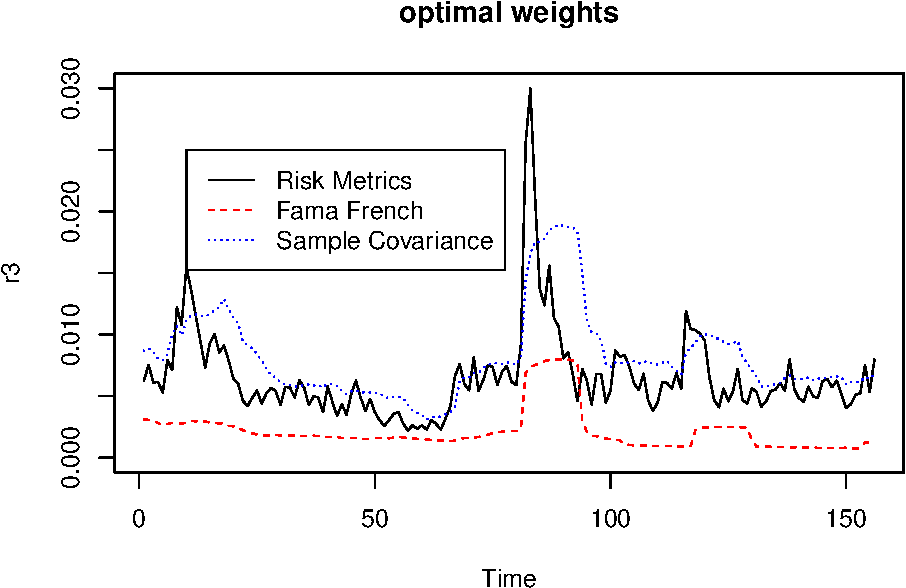
\includegraphics{hw5_files/figure-latex/unnamed-chunk-4-1.pdf}

\begin{Shaded}
\begin{Highlighting}[]
\CommentTok{# viz }
\KeywordTok{plot}\NormalTok{(r6, }\DataTypeTok{type =} \StringTok{"l"}\NormalTok{, }\DataTypeTok{ylim =} \KeywordTok{c}\NormalTok{(}\DecValTok{0}\NormalTok{, }\FloatTok{.2}\NormalTok{), }\DataTypeTok{xlab =} \StringTok{"Time"}\NormalTok{, }\DataTypeTok{ylabe =} \StringTok{"Risk"}\NormalTok{, }
     \DataTypeTok{lty =} \DecValTok{1}\NormalTok{)}
\KeywordTok{lines}\NormalTok{(r5, }\DataTypeTok{col =} \StringTok{"red"}\NormalTok{, }\DataTypeTok{lty =}\DecValTok{2}\NormalTok{ )}
\KeywordTok{lines}\NormalTok{(r4, }\DataTypeTok{col =} \StringTok{"blue"}\NormalTok{, }\DataTypeTok{lty=}\DecValTok{3}\NormalTok{)}
\KeywordTok{legend}\NormalTok{(}\DecValTok{5}\NormalTok{, }\FloatTok{.15}\NormalTok{, }\DataTypeTok{legend =} \KeywordTok{c}\NormalTok{(}\StringTok{"Risk Metrics"}\NormalTok{, }
                           \StringTok{"Fama French"}\NormalTok{, }
                           \StringTok{"Sample Covariance"}\NormalTok{), }
       \DataTypeTok{col=}\KeywordTok{c}\NormalTok{(}\StringTok{"black"}\NormalTok{, }\StringTok{"red"}\NormalTok{, }\StringTok{"blue"}\NormalTok{),}
       \DataTypeTok{lty=}\DecValTok{1}\OperatorTok{:}\DecValTok{3}\NormalTok{)}
\KeywordTok{title}\NormalTok{(}\StringTok{"equal weights"}\NormalTok{)}
\end{Highlighting}
\end{Shaded}

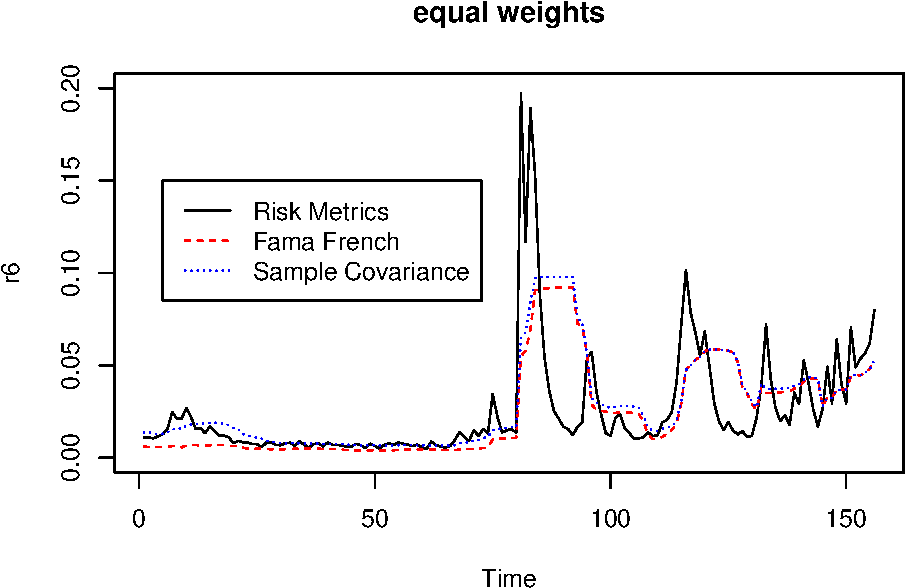
\includegraphics{hw5_files/figure-latex/unnamed-chunk-4-2.pdf}
\newpage
\singlespacing 
\end{document}
